\documentclass{beamer}
\usetheme{Warsaw}
\usepackage{amsmath, amssymb}
\usecolortheme{lily}
\setbeamertemplate{navigation symbols}{}


% boadilla seems to be the only one with enough space for stuff.compile it now it is very toxic but works

\usepackage{graphicx} % Required for inserting images
\usepackage{caption}
\usepackage{subcaption}
\usepackage{tikz}
\usepackage{pgfplots}
\usepackage{verbatim}
\usepackage{mathtools}

\pgfplotsset{compat = newest}
\usetikzlibrary{matrix}
\usepackage[dvipsnames]{xcolor}
\usetikzlibrary{perspective}

\DeclareMathOperator{\divergence}{div}
\DeclareMathOperator{\lensop}{L}
\DeclareMathOperator{\rotmatop}{R}
\DeclareMathOperator{\soop}{SO}
\newcommand*{\lens}[2]{\textcolor{darkyellow}{\lensop\left(\textcolor{black}{#1},\textcolor{black}{#2}\right)}} %
\newcommand*{\so}[1]{\soop\left(#1\right)}
\newcommand*{\rotmat}[1]{\textcolor{red}{\rotmatop\left(\textcolor{black}{#1}\right)}}
\renewcommand{\S}{\mathbb{S}}
\newcommand{\R}{\mathbb{R}}
\newcommand{\sparkles}{
\includegraphics[height=0.9em]{sparkles.png}}

% cool color

\usepackage{xcolor}
\usepackage{nicematrix}
\NiceMatrixOptions{
code-for-first-row = \color{red} ,
code-for-last-row = \color{blue} ,
code-for-first-col = \color{blue} ,
code-for-last-col = \color{blue}
}


\title{Computing CMB Temperature Fluctuations for Spherical Spaces}
\author{Adriel Matei, Béla Schneider, Javier Vela, Juš Kocutar}
\institute{University of Groningen}


\date{March 24, 2025}

\DeclareMathOperator{\cl}{cl}
\DeclareMathOperator{\rank}{r}

% Define custom headline
\setbeamertemplate{headline}{%
  \leavevmode%
  \begin{beamercolorbox}[wd=\paperwidth,ht=2.5ex,dp=1.5ex]{section in head/foot}%
    \mbox{}\hspace{.5em}\strut\insertsectionhead\mbox{}\hfill\strut  {\insertframenumber/\inserttotalframenumber}\mbox{}\strut\hspace{.5em}\mbox{}%
  \end{beamercolorbox}%
}

\setbeamercolor{block title}{fg=white, bg=purple!50!black}
\setbeamercolor{block body}{fg=black, bg=pink!20}
\setbeamercolor{titlebox}{fg=black,bg=white}

\definecolor{silver}{RGB}{192, 192, 192}
\definecolor{darkyellow}{RGB}{186, 142, 35}

\begin{document}

\section{Introduction}

 {
  \usebackgroundtemplate{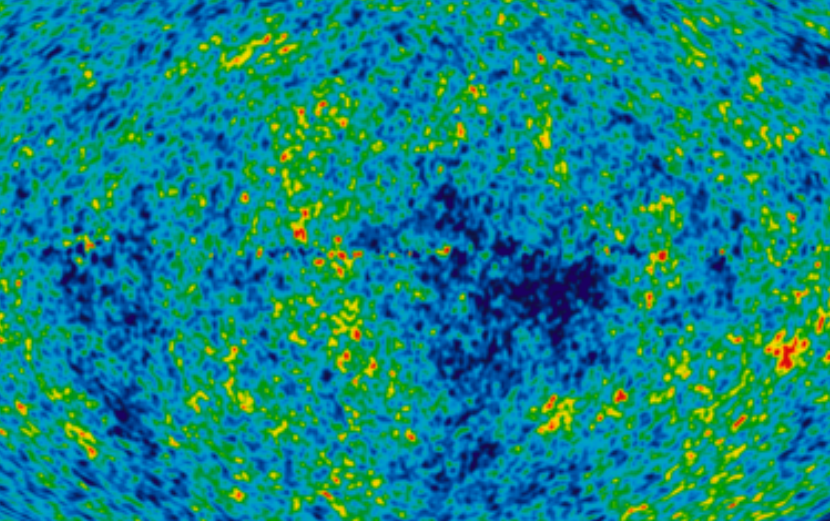
\includegraphics[height=\paperheight]{cmb.png}}
  \begin{frame}
	  \begin{beamercolorbox}[center]{titlebox}
		  \titlepage
	  \end{beamercolorbox}
  \end{frame}
 }

\section{Prerequisites}
\begin{frame}{Introduction}
	\begin{figure}[H]
		\centering
		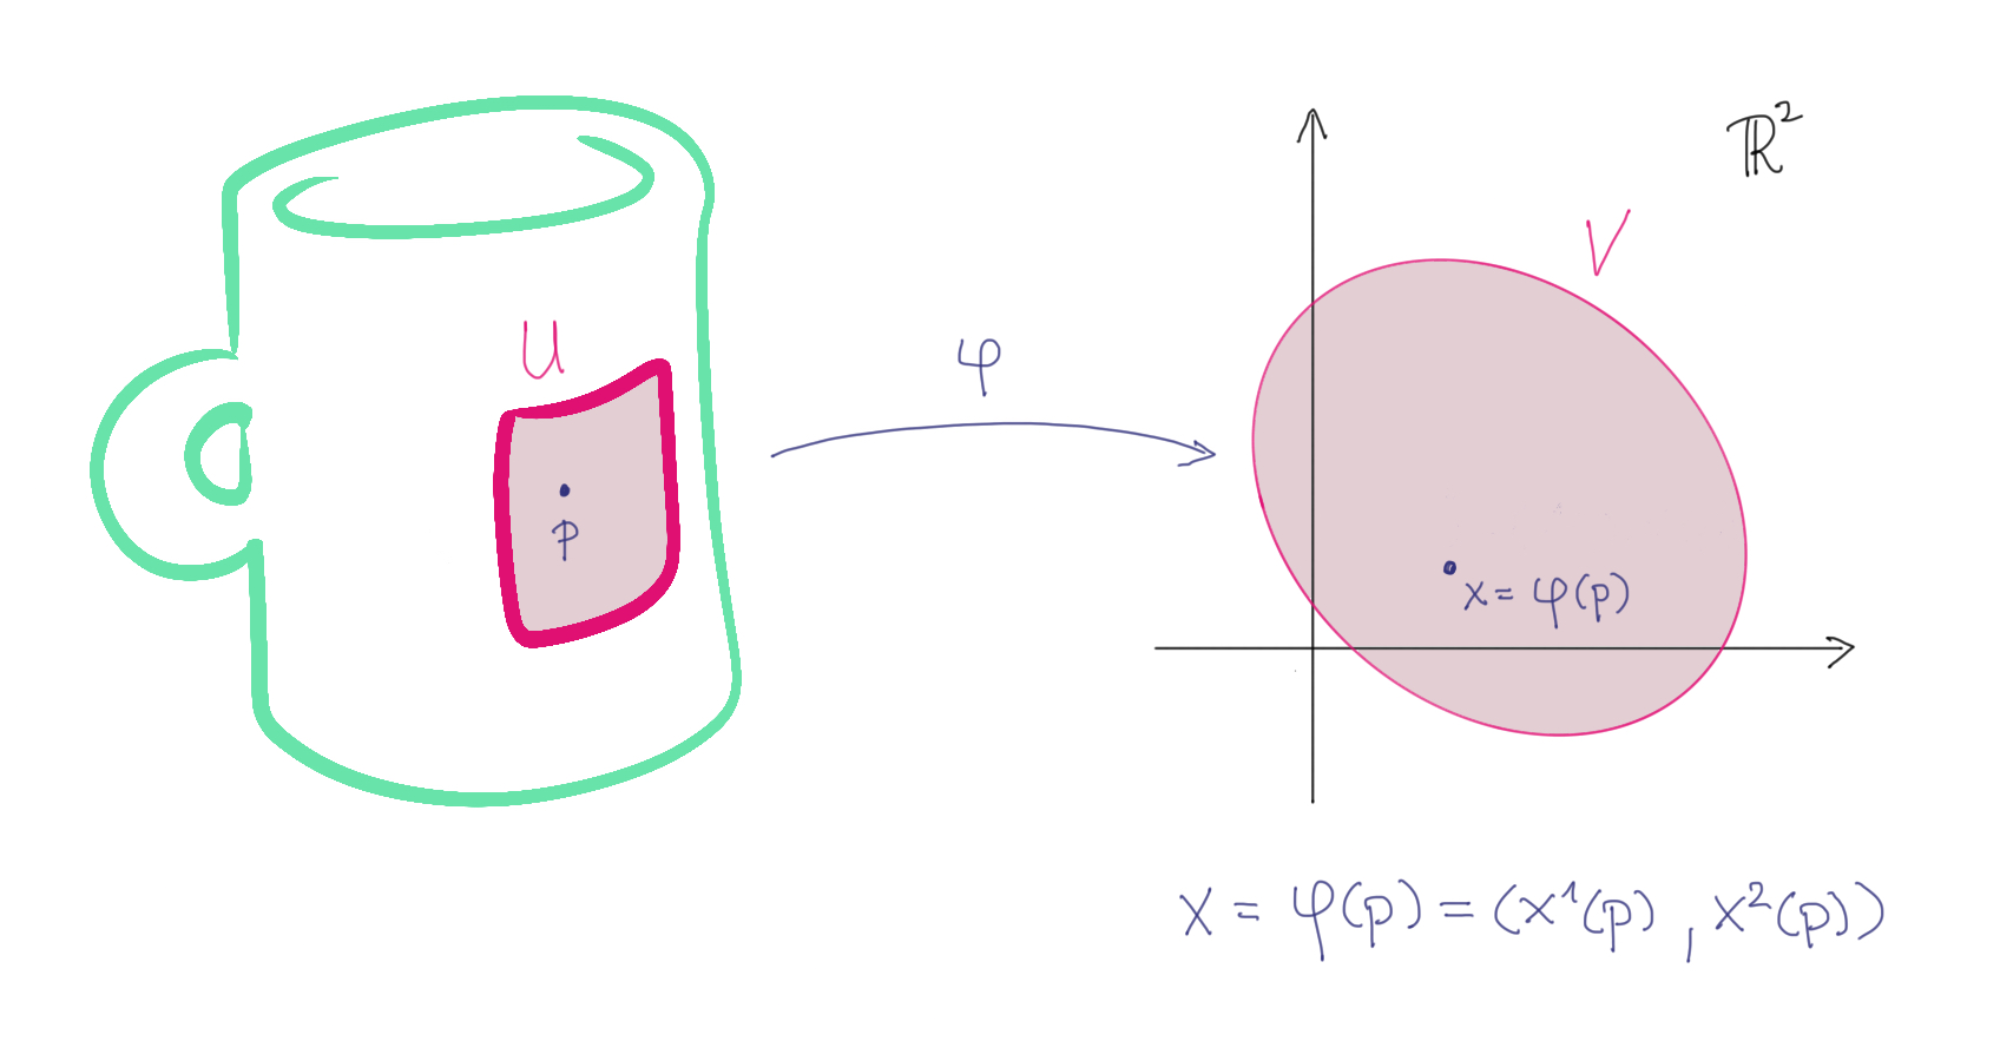
\includegraphics[width=0.5\linewidth]{mug-neighbourhoods.png}
		\caption{The prototypical example of a manifold a mug. Image source: [13]}
		\label{fig:mug-neighbourhoods}
	\end{figure}

	\begin{figure}[H]
		\centering
		%$ \captionsetup{width=.75\linewidth}
		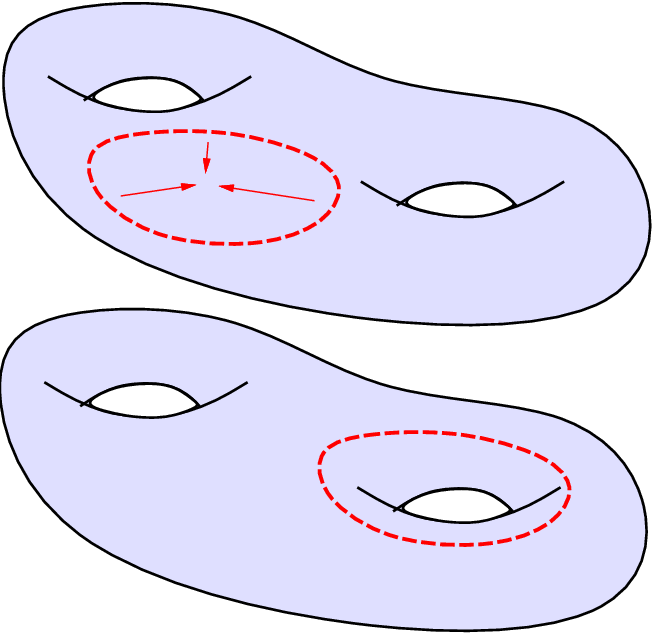
\includegraphics[width=0.2\linewidth]{Contractible loops.png}
		\caption{Diagram showing two double tori with (non)-contractible paths.  Image source[7]}
		\label{fig:CoLoop}
	\end{figure}
\end{frame}

\begin{frame}{Preliminaries- quotient groups (Put actual title later)}
	ddgagagagaga
\end{frame}

\section{The spectral geometry of hyperbolic and spherical spaces}
\begin{frame}{The Laplace-Beltrami operator}
	\begin{enumerate}
		\begin{definition}[Laplace-Beltrami operator]
			a generalization of the Laplace operator to more general spaces
			\begin{align*}
				\Delta f \coloneq \divergence \nabla f.
			\end{align*}
		\end{definition}
		\item The spectrum of this operator is a subset of $[0, \infty)$. We call it the \textcolor{blue}{\emph{spectrum}} of the manifold.
		      \pause
		\item The spectrum determines many things about the space (like its volume).
		\item When two distinct (up to isomorphism) manifolds share a spectrum, they for an \textcolor{red}{\emph{isospectral pair}}.
	\end{enumerate}
\end{frame}

\begin{comment}
\begin{frame}{Can isospectral pairs approximate your mom}
	\begin{itemize}
		\item One of the problems the paper studies is finding volume-maximizing isospectral pairs of spherical forms (i.e. the spaces we are interested in).
		\item Isospectral pairs share the order of their homotopy groups.
		\item The paper classifies spherical forms with homotopy group of order $<24$.
		\item It follows that any such isospectral pairs (with group order $<24$) are lens spaces.
	\end{itemize}
\end{frame}

\begin{frame}{Combining lenses into larger spaces}
	\begin{itemize}
		\item We can combine lens spaces by concatenating their lists of indices.
		\item Together with a computational search, the paper builds a table of the solutions for a bunch of dimensions. The general case is still an open question.
	\end{itemize}
\end{frame}
\end{comment}

{
\usebackgroundtemplate{
	
\begin{tikzpicture}
		\clip (0,0) rectangle (\paperwidth,\paperheight);
		\fill[color=silver] (\paperwidth-10pt,0) rectangle (\paperwidth,\paperheight);
		% Added
		\fill[color=silver](0,0) rectangle (10pt,\paperheight);
	\end{tikzpicture}
}

\begin{frame}{The silver lining}
	\begin{itemize}
		\item Isospectral pairs are intriguing in their own right, but they cannot occur in dimension $3$.
		\item We can thus attempt to infer the shape of our universe based on its spectrum.
	\end{itemize}
\end{frame}
}


\section{CMB Anisotropy of Spherical Spaces}

\begin{frame}[fragile]{Homogeneous Spherical Spaces}
	\begin{itemize}
		\pause
		\item Finite subgroup $\Gamma \leq \so 4.$
		      \pause
		\item The Helmholtz equation on $\textcolor{blue}{M}$ has the spectrum of the underlying manifold as its solutions, and is given by
		      \begin{align*}
			      (\Delta + E_{\textcolor{red}{\beta}}^{\textcolor{blue}{M}})\psi_{\textcolor{red}{\beta}}^{{\textcolor{blue}{M}}, i} = 0.
		      \end{align*}
		      \pause
		\item In fact $E_{\textcolor{red}{\beta}}^M = {\textcolor{red}{\beta}}^2-1$ for $\textcolor{red}{\beta} \in \mathbb{N}$. We call $\textcolor{red}{\beta}$ a wave number.
		      \pause
		\item The set of all possible wave numbers [for which a nonzero solution exists] depends on $\Gamma$ - usually a proper subset of $\mathbb{{N}}$.
		      \pause
		\item Solutions to the Helmholtz equation are calculated for each $\Gamma$ and CMB anisotropy $\textcolor{purple}{\frac{\delta T}{T}}$ computed as a sum of spherical harmonics.
	\end{itemize}
\end{frame}


\begin{comment}

\begin{frame}[fragile]{CMB Anisotropy of Homogeneous Spherical Spaces}
	\begin{itemize}
		\item If $H = \{1\}$ the set of wave numbers is $\mathbb{N}$
		\item If $H = \mathbb Z/m\mathbb Z$ for odd $m$ the set of wave numbers is $$\{1,3,\cdots, m\}\cup \{m+1, m+2, m+3, \cdots \}.$$
		\item  If $H = O^*$, the binary tetrahedral group --- a subgroup of $SO(4)$ of size 24, the set of wave numbers is $$\{ 1,7,9 \} \cup \{13,15,17,\cdots \}.$$
	\end{itemize}
\end{frame}

\end{comment}


\begin{frame}[fragile]{Homogenous Spherical Spaces --- Results}
	\begin{itemize}
		\pause
		\item For the majority of groups $\Gamma$, the anisotropies $\textcolor{purple}{\frac{\delta T}{T}}$ do not coincide with observations.
		      \pause
		\item The only groups for which they do are $\Gamma = O^*$ and $\Gamma = I^*$ — the \textcolor{red}{binary octahedral} and \textcolor{red}{binary icosahedral} groups of order 48 and 120 respectively.
		      \pause
	\end{itemize}
	\begin{figure}[H]
		\centering
		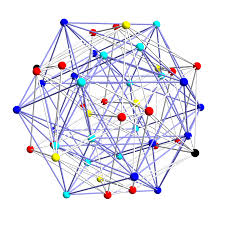
\includegraphics[width=0.4\linewidth]{binary-octahedron.png}
		\caption{Graphical representation of the binary tetrahedral group
				[5]}
	\end{figure}

\end{frame}

\section{CMB Radiation in an Inhomogeneous Spherical Space}

\begin{frame}{Inhomogeneous spherical space}

	\begin{itemize}
        \pause
		\item Manifolds of the form $\S^3/\Gamma$ with $\Gamma$ a group acting on $\S^3$.
		\item \textcolor{red}{Multi-connected} space: it has non-contractable loops.
		\item \textcolor{red}{Inhomogeneous} space: it does not look identical from every point in space.
		      \pause
		\item Fixing $|\Gamma|=8$, we have \textcolor{red}{three} multi-connected manifolds, up to equivalence: \pause
		      \begin{enumerate}
			      \item homogeneous: $N3$ and $\lens 8 1 $.
			      \item inhomogeneous: $N2 \equiv \lens 8 3 $.
		      \end{enumerate}
		      \pause
		\item Results: inhomogeneous spaces have \textcolor{red}{more variety} in the CMB anisotropies than homogeneous spaces, because the strength of anisotropy suppression is \textcolor{red}{observer dependent}.
	\end{itemize}


\end{frame}

\section{Test for anisotropy in the mean of the CMB temperature fluctuation in spherical harmonic space}

\begin{frame}{Statistical Isotropy and Hypothesis}
	\small
	\textbf{Theoretical Expectation:}\\
	From the perspective of an Earth-based observer, we can view the CMB as a function defined on the celestial sphere $\mathbb{S}^2.$\\
	\begin{itemize}
		\pause
		\item The CMB temperature fluctuations can be expanded as:
		      \[
			      \Delta T(\hat{n}) = \sum_{\ell=0}^{\infty} \sum_{m=-\ell}^{\ell} \textcolor{blue}{a_{\ell m}}  Y_{\ell m}(\hat{n})
		      \]
		      \pause
		\item If the universe is isotropic, the \textcolor{red}{mean of the harmonic coefficients} should satisfy:
		      \[
			      \langle \textcolor{blue}{a_{\ell m}}  \rangle = 0
		      \]
	\end{itemize}
	\pause
	\textbf{Key Question:}
	- Does the observed CMB data deviate from statistical isotropy?
	- If \( \langle \textcolor{blue}{a_{\ell m}} \rangle \neq 0 \), this suggests a preferred cosmic direction.
\end{frame}

\begin{frame}{Methodology: Sky Masking and the Test Statistic}
	\small
	\textbf{Challenges in Real Observations:}
	\begin{itemize}
		\item We cannot observe the full CMB sky due to foreground contamination.

		\item A \textbf{sky mask function} \( A(\hat{n}) \) removes contaminated regions, but introduces bias.
		      \pause
		\item The test statistic \( S_i \) is used, with a matrix $W$ to correct for these effects:
		      \[
			      S_i = \sum_{j} W_{ij} M_j
		      \]
	\end{itemize}
	\pause
	\textbf{Monte Carlo Simulations:}
	\begin{itemize}
		\item We generate thousands of \textbf{simulated CMB skies} assuming isotropy.
		\item Each sky has different random \( a_{\ell m} \), drawn from:
		      \[
			      \textcolor{blue}{a_{\ell m}}  \sim \mathcal{N} (0, C_\ell)
		      \]
		\item The observed WMAP data is compared against these simulations.
	\end{itemize}
\end{frame}


\begin{frame}{Results and Interpretation}
	\small
	\begin{columns}
		\column{0.5\textwidth}
		\begin{figure}
			\centering
			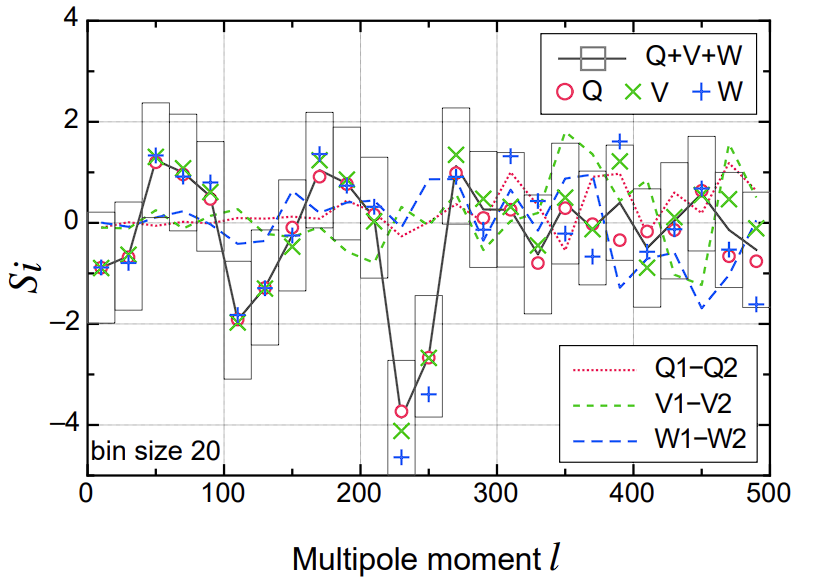
\includegraphics[width=6.2cm]{DSE-Test Graph}
			\caption{The decorrelated band mean test statistic values over multipole ranges [9].}
		\end{figure}
		\column{0.5\textwidth}
		\pause
		\textbf{Key Findings:}
		\begin{itemize}
			\item A statistically significant deviation was found in \( 221 \leq \ell \leq 240 \).
			\item This suggests a potential \textcolor{red}{preferred cosmic direction}.
		\end{itemize}
		\pause
		\textbf{Possible Explanations:}
		\begin{itemize}
			\item A real cosmological signal? → A finite universe or new physics.
			\item A systematic effect? → Technological or theory related limitations.
		\end{itemize}
	\end{columns}
\end{frame}


\section{Conclusion}
\begin{frame}{Conclusion}
	\pause
	\begin{enumerate}
		\item We can infer the \textcolor{blue}{shape} of the universe from its \textcolor{blue}{spectrum}.

		      \pause
		\item There are two homogeneous spherical manifolds obtained as $\S^3/\Gamma$ which produce CMB similar to observations.

		      \pause
		\item Inhomogeneous spherical spaces exhibit varied behavior of CMB anisotropies.

		      \pause
		\item Statistical test results suggest possibilities of \textcolor{red}{finite multi-connected} topology.
	\end{enumerate}
\end{frame}


\section{References}
\begin{frame}{References}
	\begin{itemize}
		\item [1] R. Aurich, P. Kramer, and S. Lustig. \textit{Cosmic microwave background radiation in an inhomogeneous spherical space}. Physica Scripta, 2011.
		\item [2] R. Aurich, P. Kramer, and S. Lustig. \textit{A survey of lens spaces and large-scale CMB anisotropy}. Monthly Notices of the Royal Astronomical Society, 2012.
		\item [3] R. Aurich, S. Lustig, and F. Steiner. \textit{CMB anisotropy of spherical spaces}. Classical and Quantum Gravity, 2005.
		\item [4] P. Bielewicz, K. M. G´orski, and A. J. Banday. \textit{Low-order multipole maps of cosmic microwave background anisotropy derived from WMAP}. Oxford University Press, 2004.
		\item [5]G. Egan. \textit{Symmetries and the 24-cell}. 2021. Accessed at https://www.gregegan.net/SCIENCE/24-cell/24-cell.html.
	\end{itemize}
\end{frame}


\begin{frame}{References 2 --- Electric Boogaloo}
	\begin{itemize}

		\item [6] N. Jarosik et. al. \textit{Seven-year Wilkinson Microwave Anisotropy Probe (WMAP) Observations: Sky Maps, Systematic Errors, and Basic Results}. The American Astronomical Society, 2011.
		\item [7] M. Herlihy and N. Shavit. \textit{The Topological Structure of Asynchronous Computability}. Journal of the ACM, 1996.
		\item [8] A. Ikeda. \textit{On the spectrum of a Riemannian manifold of positive constant curvature}. Osaka Journal of Mathematics, 1980.
		\item [9] D. Kashino, K. Ichiki, and T. Takeuchi. \textit{Test for anisotropy in the mean of the CMB temperature fluctuation in spherical harmonic space}. Physics Review, 2012.
		\item [10] P. Labrana. \textit{Emergent Universe Scenario and the Low CMB Multipoles}. Physical Review, 2013.
	\end{itemize}
\end{frame}

\begin{frame}{References 3 --- the References Strike Again}
	\begin{itemize}
		\item [11] E. A. Lauret and B. Linowitz. \textit{The spectral geometry of hyperbolic and spherical manifolds: analogies and open problems}. New York Journal of Mathematics, 2025.
		\item [12] R. Lehoucq, J. Weeks, J. P. Uzan, E. Gausmann, and J.P. Luminet. \textit{Eigenmodes of three-dimensional spherical spaces and their application to cosmology}. Classical and Quantum Gravity, 2002.
		\item [13] M. Serri. \textit{Analysis on Manifolds}. AMS Open Math Notes, 2025.
		\item [14] B. Tai-Dana, T. Bryson, and J. Terilla. \textit{Topology, a categorical approach}. The MIT Press, 2020.
	\end{itemize}
\end{frame}


\begin{frame}{}
	\begin{figure}[H]
		\centering
		
\includegraphics[width=.4\paperwidth]{qrcode.png}
	\end{figure}
	\begin{center}
		\huge \sparkles\: Thank You! \sparkles
	\end{center}
\end{frame}


\end{document}
